\chapter{总结与展望}
本章将对本人毕业论文相关工作进行总结与展望,总结是从当前网络协议栈兼容性方面和本用户态协议栈工作两个进行,展望是针对当前用户态协议栈系统的不足,提出几点可以在将来的研究中进行改进的设想。
\section{总结}
移动互联网和人工智能网络的兴起使得数据中心网络流量与日俱增,与此同时,在硬件设备方面网卡与物理内存带宽的飞速发展使得网络相关应用的性能瓶颈逐渐转移到传统内核网络协议栈中。学术界和工业界对网络协议栈在内核态和用户态进行了各种方式的优化,内核态网络协议栈的优化带来的性能提升有限,用户态协议栈性能较高但难以兼容现有传统网络应用,如表~\ref{tab:compare}所示,在兼容性从是否支持POSIX API、是否需要修改应用源码、是否支持Epoll等IO多路复用机制这三个方面对本工作的用户态协议栈与其他已有协议栈进行对比,可以看到本工作达到达到与Affinity-Accept、Fastsocket一样优秀的用户兼容性,并通过实验验证为Nginx等Web服务器带来的网络性能提升高于这两者。

\begin{table}[]
\centering
\caption{协议栈兼容性对比}
\label{tab:compare}
\begin{tabular}{lllp{3cm}}
\toprule[1.5pt]
\textbf{协议栈名称} & \textbf{是否支持POSIX API} & \textbf{是否需要修改应用源码} & \textbf{是否支持Epoll等IO多路复用} \\ 
\midrule[1pt]
Affinity-Accept & 是 & 不需要 & 支持 \\
MegaPipe &  否  & 需要  & 不支持 \\
Fastsocket & 是 & 不需要 & 支持 \\
mTCP & POSIX-Like & 需要 & 支持 \\
IX & 否 & 需要 & 不支持 \\
F-stack & POSIX-Like & 需要 & 支持 \\
Seastar & 否 & 需要重写应用 & 异步IO \\
\textbf{本用户态协议栈*} & 是 & 不需要 & 支持 \\
\bottomrule[1.5pt]
\end{tabular}
\end{table}

为了解决移植传统应用的兼容性,本文提出在用户态实现高性能且高度兼容性的协议栈,即传统网络应用在不需要修改任何源码的前提下就可以获得网络性能的提升。从更具体的层面上,本文在用户态协议栈的工作总结起来有如下几点:

第一,将Linux内核操作系统中网络协议栈的代码剥离出来,界定底层网卡驱动收包与网络协议栈的边界,并使用DPDK提供基于轮询IO的收发包、定时器、netdev、内存管理接口替换到原来内核协议栈中的接口,将数据包结构体sk\_buff与DPDK的mbuf整合到一起,为网络协议栈和应用提供数据缓冲支持。

第二,采用协议栈进程与网络应用进程分核的设计思路,通过DPDK提供的rte\_mempool和rte\_ring对套接字、文件描述符等资源实现资源池化管理,并进行资源预分配,减少网络高并发情况下资源不断申请、释放的性能开销。并使用有名管道和内核Epoll来实现在用户态实现Epoll相关接口以及epoll\_wait阻塞接口的唤醒机制,从而完成对IO多路复用事件通知接口。以上工作都是为在用户态实现网络应用的高度兼容性打下坚实的基础。

第三,利用LD\_PRELOAD和动态链接技术对网络应用的POSIX API进行劫持,并使用文件描述符空间预分配资源池和双向映射解决网络文件描述符和非网络文件描述符的空间分割管理问题。此外,针对当前Nginx、Lighttpd等主流网络应用服务器存在多进程等并发网络模型,对系统的CPU核资源以及执行流资源进行合理匹配,从而完成并发网络应用的支持。

第四,成功移植了Nginx、Lighttpd、Redis等主流网络应用,并将自行开发的经典网络模型服务器成功移植到本用户态协议栈上,其中包括one process per request多进程模型和基于Epoll的多线程网络模型。在Nginx、Lighttpd等Web服务器上获得超过50\%的网络性能提升,并将尾延迟降低超过90\%之多,在Redis等Key Value内存服务器上对GET操作带来超过30\%的网络性能提升,最关键是这些提升都可以在完全不需要网络应用源码的前提下直接完成。

\section{展望}

本文工作的目标是在用户态实现一个既具备高度兼容性又能带来明显网络性能提升的协议栈,解决之前高性能用户态协议栈移植网络应用成本较高的问题,达到兼容性与高性能两者的平衡。当前本用户态协议栈工作确实做到了在不需要修改源码的前提下移植网络应用,不过与mTCP等高性能协议栈相比性能不到其70\%,这也是未来本协议栈工作应该在性能方面进行更加深度的优化,以使该高度兼容的用户态协议栈具备更高的网络性能。为此,本人针对当前用户态协议栈提出如下几点改进路径:

第一,由于用户态套接字、文件描述符等大页内存资源池是多个协议栈进程共享的,这会造成rte\_ring提供的申请释放接口必须使用多生产者多消费者模式,且在高并发高吞吐流量下套接字和文件描述符资源会在多个CPU核的Cache中进行迁移,这无疑造成多进程模式下压测网络性能的降低,所以需要将套接字等资源池改变成为单个协议栈进程独享。然而由于协议栈进程通过DPDK初始化时大页内存等资源的申请只能在primary进程中进行,其他协议栈secondary进程只是获取primary申请的资源池的地址,这就导致必须将primary申请的资源池根据协议栈进程个数与资源池大小进行逻辑上的切分,即资源池中资源的申请和释放的接口会带有一个表示协议栈id的编号,而每个协议栈进程在初始化的时候都能得到自己的编号,这样在套接字资源申请时候会传递协议栈id并只能该id对应的资源池片段中申请资源,这样资源的申请与释放在协议栈进程与网络应用进程中就能按照单消费者单生产者的模式进行,减少锁竞争以及Cache迁移带来的开销。当然,该设计需要一个前提就是网络流量是较为均匀地分散到各个协议栈进程中处理,否则会造成资源池片段的使用失衡,该前提是可以通过DPDK提供的对称哈希与RSS技术来保证。

第二,当前本系统的协议栈进程只能绑定一个网络应用进程,CPU资源的利用率较低,同样运行一个协议栈执行流需要与mTCP两个协议栈执行流进行对比,这也是造成与mTCP性能对比较差的重要原因。mTCP通过pthread信号与条件变量实现在一个CPU核并发运行协议栈线程和网络应用线程,而本系统将协议栈执行流放到专用物理核上应该能为提供更强大的网络处理能力,即服务更多的网络应用并发流,所以下一步应该着手实现在对网络应用的服务质量影响较小的情况下可以让多个网络应用执行流绑定在一个协议栈进程上以及不同应用的执行流均可以绑定在同一个协议栈进程,如图~\ref{fig:distribute}所示。这就需要在用户态套接字和文件描述符资源对应的结构体中加入app\_id等字段,并用全局资源池记录下所有app\_id的相应信息,比如进程数、线程数、应用名称等。

\vspace{-10pt}
\begin{figure}[H] % use float package if you want it here
  \centering
  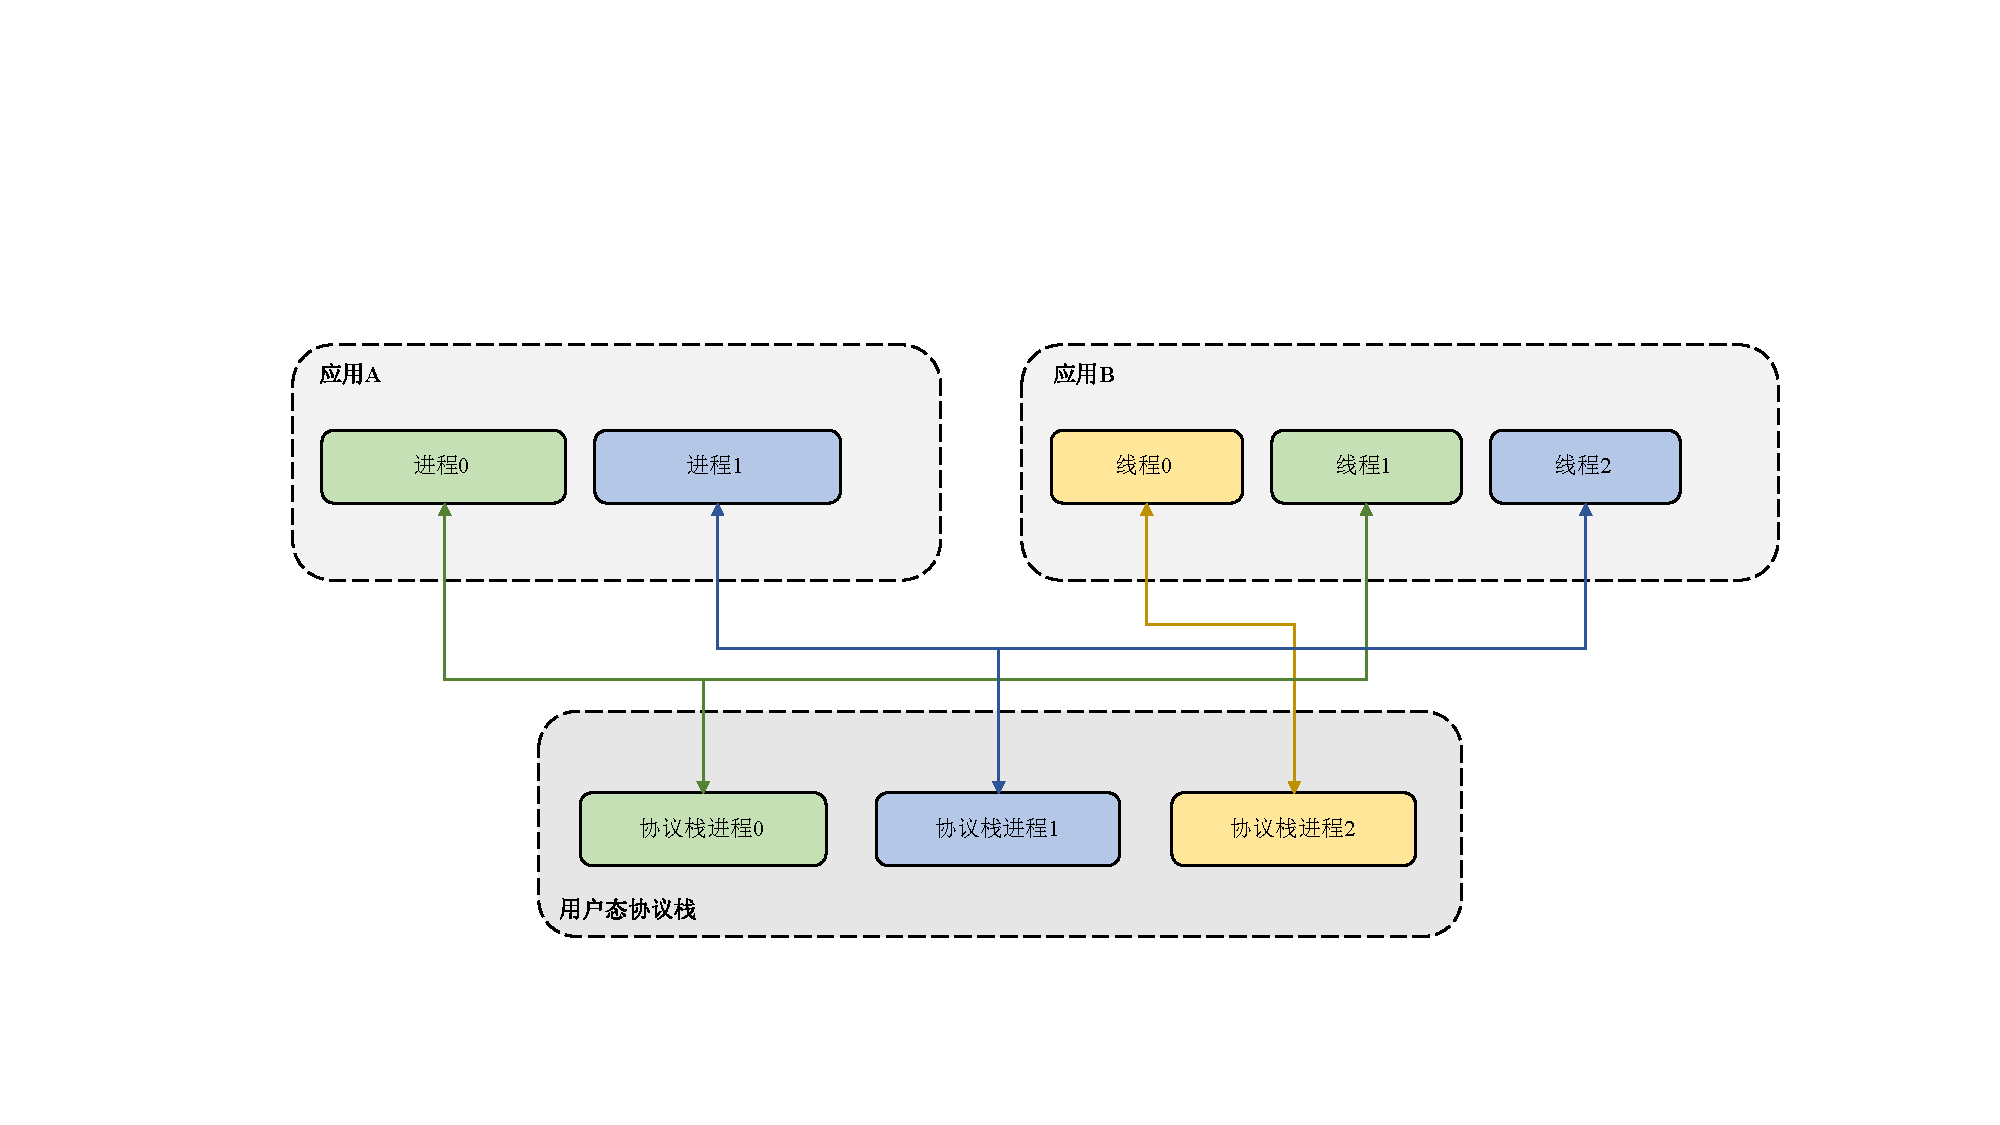
\includegraphics[width=\textwidth]{distribute}
  \caption{协议栈进程与网络执行流调度设计图}
  \label{fig:distribute}
\end{figure}
\vspace{-10pt}

第三,前两点长期稳定运行的前提需要协议栈进程本身的鲁棒性,若协议栈进程崩溃且网络应用未被通知的情况下会出现无法服务或绑定失败的异常情况,这需要系统对协议栈进程本身的运行状况进行监控。当前系统通过在协议栈primary进程建立Unix域socket而网络应用进程对其进行Unix域socket连接的方式并结合内核Epoll来完成对应用进程的异常状态的监控,若协议栈primary进程自身异常退出导致此方法无法对协议栈进程异常进行监控,所以需要将监控程序单独剥离出成为一个独立进程,该监控进程完成Unix域监听socket的建立,并在协议栈进程和网络应用进程初始化时都通过内核套接字对监控进程的Unix域监听套接字进行连接,这样当协议栈进程或应用进程异常退出后都能在监控进程中通过Epoll事件获取,此外监控进程通过内核epoll\_wait监听阻塞后并不占用CPU资源,这样所有系统监控的工作全部可以放入该监控进程模块来完成,实现系统各个模块的解耦。

